
\usepackage{fancyhdr}
\usepackage{lastpage}
\usepackage[utf8]{inputenc}

% Minted for syntax highliting
\usepackage{minted}
\usemintedstyle{tango}

% Headers/footers styling
\pagestyle{fancy}
\fancyhf{}
\renewcommand{\headrulewidth}{0pt}

% Footer
\lfoot{ID1019}
\cfoot{KTH}
\rfoot{\thepage \hspace{1pt} / \pageref{LastPage}}

%\newcommand{\defaultpagestyle}{\thispagestyle{plain}}
\newcommand{\defaultpagestyle}{\thispagestyle{fancy}}


\title[ID1019 Trees]{Trees}


\author{Johan Montelius}
\institute{KTH}
\date{\semester}

\begin{document}

\begin{frame}
\titlepage
\end{frame}

\begin{frame}{compound structures}

Compound data structures in Erlang:

\begin{itemize}
 \item {\bf tuples:} {\tt \{student, ``Sune Mangs'', cinte, 2012,  sunem\}}
 \item {\bf lists:} {\tt [sunem, joed, sueb, anng]}
\end{itemize}
\end{frame}


\begin{frame}{lists}

We could implement lists using tuples:

\pause

\begin{code}
   <list> ::=  & nil | \\
               & \{cons, <structure>, <list> \}
\end{code}


\pause \vspace{20pt}
{\tt [foo, bar, zot]}

\pause \vspace{10pt}
{\tt [foo | [ bar | [zot | [] ] ] ] }

\pause \vspace{10pt}
{\tt \{cons, foo, \{cons, bar, \{cons, zot, nil\}\}\}}

\end{frame}


\begin{frame}{lists}

\pause Lists gives us a convenient syntax ... \pause once you get use to it.
\vspace{20pt}

\pause Lists are handled more efficiently by the compiler and run-time system.

\vspace{20pt}
\pause Important to understand when to use lists and when to use tuples.

\end{frame}

\begin{frame}[fragile]{nth element}

Return the n'th element from a list of three:

\pause 
\begin{verbatim}
nth_l(1, [R|_]) -> R;
nth_l(2, [_,R|_]) -> R;
nth_l(3, [_,_,R|_]) -> R.
\end{verbatim}

\pause Return the n'th element from a tuple of three:
\pause

\begin{verbatim}
nth_t(1, {R,_,_}) -> R;
nth_t(2, {_,R,_}) -> R;
nth_t(3, {_,_,R}) -> R.
\end{verbatim}

\end{frame}

\begin{frame}[fragile]{nth element}

Return the n'th element from a list:

\pause 
\begin{verbatim}
nth(1, [R|_]) -> R;
nth(N, [_|T]) -> nth(N-1, T).
\end{verbatim}

\end{frame}


\begin{frame}{nth element}

\begin{itemize}
  \item {\tt element(N, Tuple):} return the n'th element in the tuple
  \item {\tt lists:nth(N, List):} return the n'th element of the list
\end{itemize}

\end{frame}

\begin{frame}{n'th benchmark}
Benchmark different versions of n'th:
 \begin{figure}
  \centering
  \includegraphics[height=200pt]{nth.png}
  \caption{Execution time in ms of 100.000 calls}
 \end{figure}

\end{frame}

\begin{frame}[fragile]{copying}

Assume we represent students by a tuple {\tt \{student, Name, Prg, Year, Id\}} and we want to change program.

\pause
\begin{verbatim}
new_prgm({student, Name, _, Year, Id}, New) -> \end{verbatim}\pause\begin{verbatim}
     {student, Name, New, Year, Id}.
\end{verbatim}

\pause

How costly is this operations?

\vspace{10pt}
{\em Important to understand on what the cost depends on.}

\end{frame}


\begin{frame}{copying}

\end{frame}

\begin{frame}{when to use what}

Represent the following information using ether a list, tuple, number or atom.
                   
\begin{itemize}
\item a playing card: ace of club, king of hearts etc
\item a deck of playing cards
\item a car manufacturer: Volvo, Saab, Audi, \ldots
\item a year: 1984, 2001
\item a description of a car: maker, model, year
\item a phone number: +46-709757802
\item a course with an id, name, course responsible etc
\item a student with a number of courses two which she is enrolled
\end{itemize}

\end{frame}

\begin{frame}[fragile]{member of a list}
Assume we have a list of tuples {\tt \{card, heart, 7\}} representing playing cards. 
\pause

\vspace{10pt}
Implement a function that checks if a given card is in a deck of cards and returns {\tt yes}, or {\tt no}.

\begin{verbatim}
 member(_, []) -> ...;
 member(Card, [...|_]) -> ...;
 member(Card, [_|Rest]) -> ...;
\end{verbatim}

\end{frame}

\begin{frame}[fragile]{trees}

\pause How do we represent a binary tree?


\vspace{10pt}
\pause How do we represent a leaf node?

\vspace{10pt}
{\tt \{leaf, Value\}}

\vspace{20pt}
\pause How do we represent a branch node?

\vspace{10pt}
{\tt \{node, Value, Left, Right\}}

\vspace{10pt}
\pause How do we represent an empty tree?

\vspace{10pt}
{\tt nil}


\vspace{10pt}

\begin{verbatim}
  Tree = {node, b, {leaf, a}, {leaf, c}}
\end{verbatim}


\end{frame}


\begin{frame}{what is happening}

{\tt T = \{node, 38, \{leaf, 42\}, \{leaf, 34\}\}}

\pause \vspace{20pt}

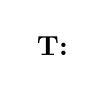
\begin{tikzpicture}[scale=0.4]


 \leaf{10}{5}{42}
 \pause 
 \leaf{6}{3}{34}

 \pause
 \branch{0.5}{8}{38}
 \pause
 \branchleft{0.5}{8}{10}{5}
 \pause
 \branchright{0.5}{8}{6}{3}

 \node at (0,8) {{\bf T:} }; 

\end{tikzpicture}

\end{frame}

\begin{frame}{what is happening}

\begin{code}
  Z = &\{node, 40, \{leaf, 42\} \{leaf, 39\}\},\\
  T = &\{node, 38, Z, \{leaf, 34\}\}
\end{code}
\pause \vspace{20pt}

\begin{tikzpicture}[scale=0.4]

 \pause 
 \leaf{16}{6}{42}
 \pause 
 \leaf{16}{3}{39}

 \pause 
 \branch{10}{8}{40}

 \pause
 \branchleft{10}{8}{16}{6}
 \pause
 \branchright{10}{8}{16}{3}

 \node at (9.5,8) {{\bf Z:} }; 

 \pause
 \leaf{6}{3}{34}

 \pause
 \branch{0.5}{8}{38}
 \pause
 \branchleft{0.5}{8}{9}{8}
 \pause
 \branchright{0.5}{8}{6}{3}

 \node at (0,8) {{\bf T:} }; 

\end{tikzpicture}

\end{frame}


\begin{frame}[fragile]{search a tree}

Given a tree, implement a function that searches for a given number,
returning {\tt yes} or {\tt no} depending on if the number is in the
tree or not.

\pause\vspace{20pt}

\begin{verbatim}
member(N, nil) -> no;
member(N, {leaf, ...}) -> yes;
member(_, {leaf, ...}) -> no;
\end{verbatim}
\pause
\begin{verbatim}
member(N, {node, ..., ..., ...}) -> yes;
\end{verbatim}
\pause

\begin{verbatim}
member(N, {node, _, Left, Right}) -> 
          case ...  of
             yes -> yes;
             no -> ....
          end.
\end{verbatim}

\pause\vspace{20pt}
What is the asymptotic time complexity of this function?
\end{frame}


\begin{frame}[fragile]{ordered tree}

How is the situation changed if the tree is ordered, smaller elements to the left and larger to the right?

\pause\vspace{20pt}

\begin{verbatim}
member(N, nil) -> no;
member(N, {leaf, ...}) -> yes;
member(_, {leaf, ...}) -> no;
member(N, {node, ..., ..., ...}) -> yes;
\end{verbatim}
\pause
\begin{verbatim}
member(N, {node, V, Left, Right}) -> 
          if 
             N < V -> ...;
             true -> ...
          end.
\end{verbatim}

\pause  What is the asymptotic time complexity of this function? {\em Assume that the tree is balanced.}

\end{frame}

\begin{frame}{key-value look-up}
Assume that we have an ordered tree of key-value pairs:

\begin{code}
  T = \{node,&k, 38,\\
             &\{node, b, 34,&nil, nil\},\\
             &\{node, o, 40,&\{node, l, 42, nil, nil\}, \\
                           &&\{node, q, 39, nil, nil\}\}\}\\

\end{code}

\vspace{20pt}No special leaf nodes, empty branch is represented by {\tt nil}.

\end{frame}

\begin{frame}[fragile]{lookup in order tree}

\pause\vspace{10pt}
How would we implement a function that searched for a given key and
returned {\tt \{value, Value\}} if found and {\tt no} otherwise?
\vspace{20pt}\pause

\begin{verbatim}
lookup(Key, nil) -> ...;
\end{verbatim}
\pause
\begin{verbatim}
lookup(Key, {node, Key, ..., ..., ...}) -> ...;
\end{verbatim}
\pause
\begin{verbatim}
lookup(Key, {node, K, _, Left, Right}) -> 
          if 
             Key < K -> ...;
             true -> ...
          end.
\end{verbatim}


\end{frame}



\begin{frame}[fragile]{modify an element}

\begin{verbatim}
modify(_, _, nil) -> nil;
\end{verbatim}
\pause
\begin{verbatim}
modify(Key, Val, {node, Key, _, Left, Right}) -> 
    {node, Key, Val, Left, Right};
\end{verbatim}
\pause
\begin{verbatim}
modify(Key, Val, {node, K, V, Left, Right}) -> 
    if 
       Key < K ->  
           {node, K, V, ..., Right};
       true  -> 
           {node, K, V, Left, ...}
    end.
\end{verbatim}

\end{frame}


\begin{frame}[fragile]{insert}

Same assumptions, how do we implement {\tt insert(Key, Value, Tree)} (assuming it does not exists)?

\pause\vspace{20pt}

\begin{verbatim}
insert(Key, Value, nil) -> ...;
\end{verbatim}
\pause
\begin{verbatim}
insert(Key, Value, {node, K, V, Left, Right}) -> 
          if 
             Key < K -> ...;
             true -> ...
          end.
\end{verbatim}

\end{frame}


\begin{frame}[fragile]{delete}

Same assumptions, how do we implement {\tt delete(Item, Tree)} (assuming it does exists)?

\pause\vspace{20pt}

\begin{verbatim}
delete(Key, {node, Key, _, nil, nil}) -> ...;
\end{verbatim}
\pause
\begin{verbatim}
delete(Key, {node, Key, _, nil, Right}) -> ...;
\end{verbatim}
\pause
\begin{verbatim}
delete(Key, {node, Key, _, Left, nil}) -> ...;
\end{verbatim}
\pause
\begin{verbatim}
delete(Key, {node, Key, _, Left, Right}) -> 
            :
\end{verbatim}
\pause
\begin{verbatim}
delete(Key, Value, {node, K, V, Left, Right}) -> 
          if 
             Key < K -> ...;
             true -> ...
          end.
\end{verbatim}
\end{frame}

\begin{frame}[fragile]{deleting a element}

\pause Algorithm first - then implement.

\pause
\begin{verbatim}
delete(Key, {node, Key, _, Left, Right}) -> 
            {K, V} = ....,
            Deleted = ...
            {node, ..., ..., ..., ...};
\end{verbatim}

\end{frame}



\begin{frame}{Summary}

\vspace{40pt}\hspace{80pt}Trees

\end{frame}


\end{document}


